\documentclass[twoside]{book}

% Packages required by doxygen
\usepackage{fixltx2e}
\usepackage{calc}
\usepackage{doxygen}
\usepackage[export]{adjustbox} % also loads graphicx
\usepackage{graphicx}
\usepackage[utf8]{inputenc}
\usepackage{makeidx}
\usepackage{multicol}
\usepackage{multirow}
\PassOptionsToPackage{warn}{textcomp}
\usepackage{textcomp}
\usepackage[nointegrals]{wasysym}
\usepackage[table]{xcolor}

% NLS support packages
\usepackage[T2A]{fontenc}
\usepackage[russian]{babel}

% Font selection
\usepackage[T1]{fontenc}
\usepackage[scaled=.90]{helvet}
\usepackage{courier}
\usepackage{amssymb}
\usepackage{sectsty}
\renewcommand{\familydefault}{\sfdefault}
\allsectionsfont{%
  \fontseries{bc}\selectfont%
  \color{darkgray}%
}
\renewcommand{\DoxyLabelFont}{%
  \fontseries{bc}\selectfont%
  \color{darkgray}%
}
\newcommand{\+}{\discretionary{\mbox{\scriptsize$\hookleftarrow$}}{}{}}

% Page & text layout
\usepackage{geometry}
\geometry{%
  a4paper,%
  top=2.5cm,%
  bottom=2.5cm,%
  left=2.5cm,%
  right=2.5cm%
}
\tolerance=750
\hfuzz=15pt
\hbadness=750
\setlength{\emergencystretch}{15pt}
\setlength{\parindent}{0cm}
\setlength{\parskip}{3ex plus 2ex minus 2ex}
\makeatletter
\renewcommand{\paragraph}{%
  \@startsection{paragraph}{4}{0ex}{-1.0ex}{1.0ex}{%
    \normalfont\normalsize\bfseries\SS@parafont%
  }%
}
\renewcommand{\subparagraph}{%
  \@startsection{subparagraph}{5}{0ex}{-1.0ex}{1.0ex}{%
    \normalfont\normalsize\bfseries\SS@subparafont%
  }%
}
\makeatother

% Headers & footers
\usepackage{fancyhdr}
\pagestyle{fancyplain}
\fancyhead[LE]{\fancyplain{}{\bfseries\thepage}}
\fancyhead[CE]{\fancyplain{}{}}
\fancyhead[RE]{\fancyplain{}{\bfseries\leftmark}}
\fancyhead[LO]{\fancyplain{}{\bfseries\rightmark}}
\fancyhead[CO]{\fancyplain{}{}}
\fancyhead[RO]{\fancyplain{}{\bfseries\thepage}}
\fancyfoot[LE]{\fancyplain{}{}}
\fancyfoot[CE]{\fancyplain{}{}}
\fancyfoot[RE]{\fancyplain{}{\bfseries\scriptsize Создано системой Doxygen }}
\fancyfoot[LO]{\fancyplain{}{\bfseries\scriptsize Создано системой Doxygen }}
\fancyfoot[CO]{\fancyplain{}{}}
\fancyfoot[RO]{\fancyplain{}{}}
\renewcommand{\footrulewidth}{0.4pt}
\renewcommand{\chaptermark}[1]{%
  \markboth{#1}{}%
}
\renewcommand{\sectionmark}[1]{%
  \markright{\thesection\ #1}%
}

% Indices & bibliography
\usepackage{natbib}
\usepackage[titles]{tocloft}
\setcounter{tocdepth}{3}
\setcounter{secnumdepth}{5}
\makeindex

% Hyperlinks (required, but should be loaded last)
\usepackage{ifpdf}
\ifpdf
  \usepackage[pdftex,pagebackref=true]{hyperref}
\else
  \usepackage[ps2pdf,pagebackref=true]{hyperref}
\fi
\hypersetup{%
  colorlinks=true,%
  linkcolor=blue,%
  citecolor=blue,%
  unicode%
}

% Custom commands
\newcommand{\clearemptydoublepage}{%
  \newpage{\pagestyle{empty}\cleardoublepage}%
}

\usepackage{caption}
\captionsetup{labelsep=space,justification=centering,font={bf},singlelinecheck=off,skip=4pt,position=top}

%===== C O N T E N T S =====

\begin{document}

% Titlepage & ToC
\hypersetup{pageanchor=false,
             bookmarksnumbered=true,
             pdfencoding=unicode
            }
\pagenumbering{alph}
\begin{titlepage}
\vspace*{7cm}
\begin{center}%
{\Large Lab-\/2 \\[1ex]\large v0.\+1.\+0 }\\
\vspace*{1cm}
{\large Создано системой Doxygen 1.8.13}\\
\end{center}
\end{titlepage}
\clearemptydoublepage
\pagenumbering{roman}
\tableofcontents
\clearemptydoublepage
\pagenumbering{arabic}
\hypersetup{pageanchor=true}

%--- Begin generated contents ---
\chapter{Алфавитный указатель пространств имен}
\section{Пакеты}
Полный список документированных пакетов.\begin{DoxyCompactList}
\item\contentsline{section}{\hyperlink{namespace_lab2}{Lab2} }{\pageref{namespace_lab2}}{}
\end{DoxyCompactList}

\chapter{Иерархический список классов}
\section{Иерархия классов}
Иерархия классов.\begin{DoxyCompactList}
\item \contentsline{section}{Lab2.\+Geometric\+Figure}{\pageref{class_lab2_1_1_geometric_figure}}{}
\begin{DoxyCompactList}
\item \contentsline{section}{Lab2.\+Circle}{\pageref{class_lab2_1_1_circle}}{}
\item \contentsline{section}{Lab2.\+Rectangle}{\pageref{class_lab2_1_1_rectangle}}{}
\begin{DoxyCompactList}
\item \contentsline{section}{Lab2.\+Square}{\pageref{class_lab2_1_1_square}}{}
\end{DoxyCompactList}
\end{DoxyCompactList}
\item \contentsline{section}{Lab2.\+I\+Print}{\pageref{interface_lab2_1_1_i_print}}{}
\begin{DoxyCompactList}
\item \contentsline{section}{Lab2.\+Circle}{\pageref{class_lab2_1_1_circle}}{}
\item \contentsline{section}{Lab2.\+Rectangle}{\pageref{class_lab2_1_1_rectangle}}{}
\end{DoxyCompactList}
\item \contentsline{section}{Lab2.\+Program}{\pageref{class_lab2_1_1_program}}{}
\item \contentsline{section}{Lab2.\+Program.\+S\+T\+A\+TE}{\pageref{class_lab2_1_1_program_1_1_s_t_a_t_e}}{}
\end{DoxyCompactList}

\chapter{Алфавитный указатель классов}
\section{Классы}
Классы с их кратким описанием.\begin{DoxyCompactList}
\item\contentsline{section}{\hyperlink{class_lab1_1_1_program}{Lab1.\+Program} }{\pageref{class_lab1_1_1_program}}{}
\end{DoxyCompactList}

\chapter{Список файлов}
\section{Файлы}
Полный список файлов.\begin{DoxyCompactList}
\item\contentsline{section}{\hyperlink{_program_8cs}{Program.\+cs} }{\pageref{_program_8cs}}{}
\end{DoxyCompactList}

\chapter{Пространства имен}
\hypertarget{namespace_lab2}{}\section{Пространство имен Lab2}
\label{namespace_lab2}\index{Lab2@{Lab2}}
\subsection*{Классы}
\begin{DoxyCompactItemize}
\item 
class \hyperlink{class_lab2_1_1_circle}{Circle}
\item 
class \hyperlink{class_lab2_1_1_geometric_figure}{Geometric\+Figure}
\item 
interface \hyperlink{interface_lab2_1_1_i_print}{I\+Print}
\item 
class \hyperlink{class_lab2_1_1_program}{Program}
\item 
class \hyperlink{class_lab2_1_1_rectangle}{Rectangle}
\item 
class \hyperlink{class_lab2_1_1_square}{Square}
\end{DoxyCompactItemize}

\chapter{Классы}
\hypertarget{class_lab2_1_1_circle}{}\section{Класс Lab2.\+Circle}
\label{class_lab2_1_1_circle}\index{Lab2.\+Circle@{Lab2.\+Circle}}
Граф наследования\+:Lab2.\+Circle\+:\begin{figure}[H]
\begin{center}
\leavevmode
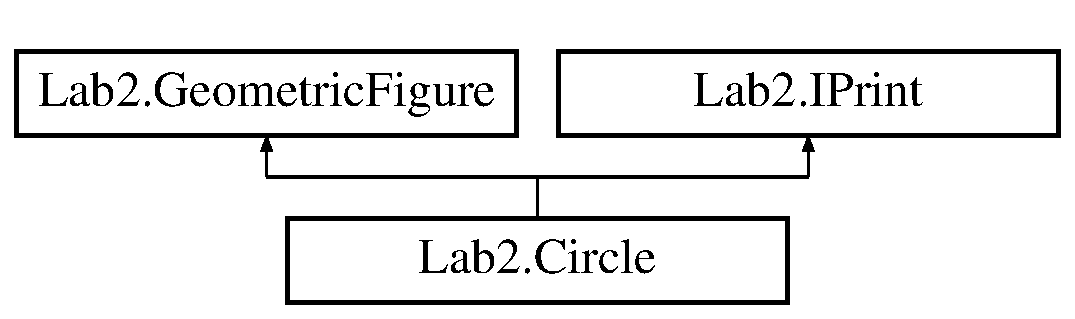
\includegraphics[height=2.000000cm]{class_lab2_1_1_circle}
\end{center}
\end{figure}
\subsection*{Открытые члены}
\begin{DoxyCompactItemize}
\item 
\hyperlink{class_lab2_1_1_circle_ac95d3e44e178cf6199237fc74698465c}{Circle} (double radius)
\item 
override double \hyperlink{class_lab2_1_1_circle_afe38ef7cc9ce4b02a6e640d3029e5962}{Area} ()
\item 
override string \hyperlink{class_lab2_1_1_circle_ab2ed9c25791cb878a8a8d8857786917d}{To\+String} ()
\item 
void \hyperlink{class_lab2_1_1_circle_a300cdfbc89e35dadfdcd35ff085ffc13}{Print} ()
\end{DoxyCompactItemize}
\subsection*{Открытые атрибуты}
\begin{DoxyCompactItemize}
\item 
\mbox{\Hypertarget{class_lab2_1_1_circle_a5a40103bb404c90294370219a5cec078}\label{class_lab2_1_1_circle_a5a40103bb404c90294370219a5cec078}} 
double \hyperlink{class_lab2_1_1_circle_a5a40103bb404c90294370219a5cec078}{r} = 0
\begin{DoxyCompactList}\small\item\em Радиус \end{DoxyCompactList}\end{DoxyCompactItemize}


\subsection{Подробное описание}
Класс круга 

\subsection{Конструктор(ы)}
\mbox{\Hypertarget{class_lab2_1_1_circle_ac95d3e44e178cf6199237fc74698465c}\label{class_lab2_1_1_circle_ac95d3e44e178cf6199237fc74698465c}} 
\index{Lab2\+::\+Circle@{Lab2\+::\+Circle}!Circle@{Circle}}
\index{Circle@{Circle}!Lab2\+::\+Circle@{Lab2\+::\+Circle}}
\subsubsection{\texorpdfstring{Circle()}{Circle()}}
{\footnotesize\ttfamily Lab2.\+Circle.\+Circle (\begin{DoxyParamCaption}\item[{double}]{radius }\end{DoxyParamCaption})}

Конструктор класса 
\begin{DoxyParams}{Аргументы}
{\em double} & radus Задает фигиру \\
\hline
\end{DoxyParams}


\subsection{Методы}
\mbox{\Hypertarget{class_lab2_1_1_circle_afe38ef7cc9ce4b02a6e640d3029e5962}\label{class_lab2_1_1_circle_afe38ef7cc9ce4b02a6e640d3029e5962}} 
\index{Lab2\+::\+Circle@{Lab2\+::\+Circle}!Area@{Area}}
\index{Area@{Area}!Lab2\+::\+Circle@{Lab2\+::\+Circle}}
\subsubsection{\texorpdfstring{Area()}{Area()}}
{\footnotesize\ttfamily override double Lab2.\+Circle.\+Area (\begin{DoxyParamCaption}{ }\end{DoxyParamCaption})\hspace{0.3cm}{\ttfamily [virtual]}}

Вычисляет площадь фигуры 

Замещает \hyperlink{class_lab2_1_1_geometric_figure}{Lab2.\+Geometric\+Figure}.

\mbox{\Hypertarget{class_lab2_1_1_circle_a300cdfbc89e35dadfdcd35ff085ffc13}\label{class_lab2_1_1_circle_a300cdfbc89e35dadfdcd35ff085ffc13}} 
\index{Lab2\+::\+Circle@{Lab2\+::\+Circle}!Print@{Print}}
\index{Print@{Print}!Lab2\+::\+Circle@{Lab2\+::\+Circle}}
\subsubsection{\texorpdfstring{Print()}{Print()}}
{\footnotesize\ttfamily void Lab2.\+Circle.\+Print (\begin{DoxyParamCaption}{ }\end{DoxyParamCaption})}

Напечатать основную информацию об объекте в консоль 

Замещает \hyperlink{interface_lab2_1_1_i_print}{Lab2.\+I\+Print}.

\mbox{\Hypertarget{class_lab2_1_1_circle_ab2ed9c25791cb878a8a8d8857786917d}\label{class_lab2_1_1_circle_ab2ed9c25791cb878a8a8d8857786917d}} 
\index{Lab2\+::\+Circle@{Lab2\+::\+Circle}!To\+String@{To\+String}}
\index{To\+String@{To\+String}!Lab2\+::\+Circle@{Lab2\+::\+Circle}}
\subsubsection{\texorpdfstring{To\+String()}{ToString()}}
{\footnotesize\ttfamily override string Lab2.\+Circle.\+To\+String (\begin{DoxyParamCaption}{ }\end{DoxyParamCaption})\hspace{0.3cm}{\ttfamily [virtual]}}

Приведение к строке \begin{DoxyReturn}{Возвращает}
string Основная информация об объекте 
\end{DoxyReturn}


Замещает \hyperlink{class_lab2_1_1_geometric_figure}{Lab2.\+Geometric\+Figure}.



Объявления и описания членов класса находятся в файле\+:\begin{DoxyCompactItemize}
\item 
Program.\+cs\end{DoxyCompactItemize}

\hypertarget{class_lab2_1_1_geometric_figure}{}\section{Класс Lab2.\+Geometric\+Figure}
\label{class_lab2_1_1_geometric_figure}\index{Lab2.\+Geometric\+Figure@{Lab2.\+Geometric\+Figure}}
Граф наследования\+:Lab2.\+Geometric\+Figure\+:\begin{figure}[H]
\begin{center}
\leavevmode
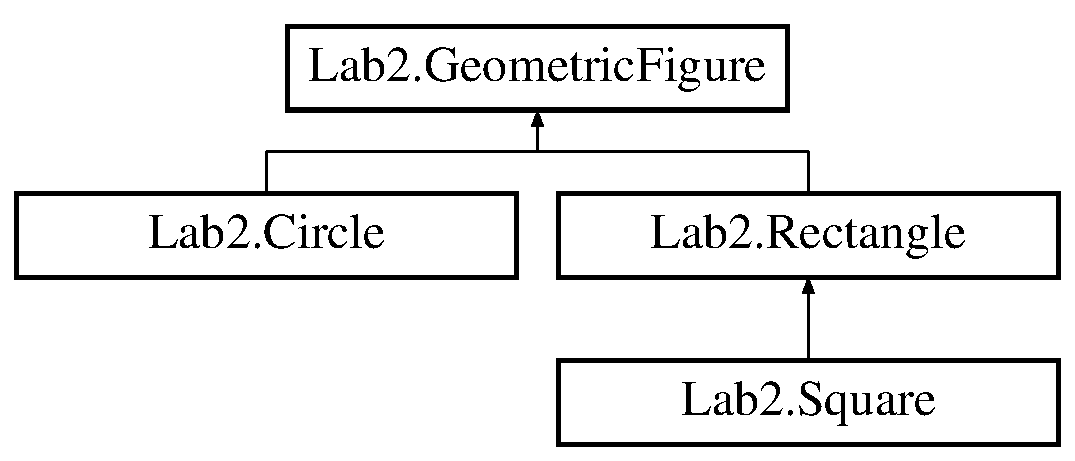
\includegraphics[height=3.000000cm]{class_lab2_1_1_geometric_figure}
\end{center}
\end{figure}
\subsection*{Открытые члены}
\begin{DoxyCompactItemize}
\item 
abstract double \hyperlink{class_lab2_1_1_geometric_figure_aeb0853b133cedd1d23f5d8a1d73af8a8}{Area} ()
\item 
abstract override string \hyperlink{class_lab2_1_1_geometric_figure_a2f466edc438f43540ead2bc66925ef0a}{To\+String} ()
\end{DoxyCompactItemize}


\subsection{Подробное описание}
Абстрактный класс фигуры 

\subsection{Методы}
\mbox{\Hypertarget{class_lab2_1_1_geometric_figure_aeb0853b133cedd1d23f5d8a1d73af8a8}\label{class_lab2_1_1_geometric_figure_aeb0853b133cedd1d23f5d8a1d73af8a8}} 
\index{Lab2\+::\+Geometric\+Figure@{Lab2\+::\+Geometric\+Figure}!Area@{Area}}
\index{Area@{Area}!Lab2\+::\+Geometric\+Figure@{Lab2\+::\+Geometric\+Figure}}
\subsubsection{\texorpdfstring{Area()}{Area()}}
{\footnotesize\ttfamily abstract double Lab2.\+Geometric\+Figure.\+Area (\begin{DoxyParamCaption}{ }\end{DoxyParamCaption})\hspace{0.3cm}{\ttfamily [pure virtual]}}



Замещается в \hyperlink{class_lab2_1_1_circle_afe38ef7cc9ce4b02a6e640d3029e5962}{Lab2.\+Circle} и \hyperlink{class_lab2_1_1_rectangle_a3a44a2229aaec3be07a35eb6a167b100}{Lab2.\+Rectangle}.

\mbox{\Hypertarget{class_lab2_1_1_geometric_figure_a2f466edc438f43540ead2bc66925ef0a}\label{class_lab2_1_1_geometric_figure_a2f466edc438f43540ead2bc66925ef0a}} 
\index{Lab2\+::\+Geometric\+Figure@{Lab2\+::\+Geometric\+Figure}!To\+String@{To\+String}}
\index{To\+String@{To\+String}!Lab2\+::\+Geometric\+Figure@{Lab2\+::\+Geometric\+Figure}}
\subsubsection{\texorpdfstring{To\+String()}{ToString()}}
{\footnotesize\ttfamily abstract override string Lab2.\+Geometric\+Figure.\+To\+String (\begin{DoxyParamCaption}{ }\end{DoxyParamCaption})\hspace{0.3cm}{\ttfamily [pure virtual]}}



Замещается в \hyperlink{class_lab2_1_1_circle_ab2ed9c25791cb878a8a8d8857786917d}{Lab2.\+Circle}, \hyperlink{class_lab2_1_1_square_ac43e17280bb521a3466a38ec0e4742eb}{Lab2.\+Square} и \hyperlink{class_lab2_1_1_rectangle_a6c03cbd28985951c1c167b51ed47cdd4}{Lab2.\+Rectangle}.



Объявления и описания членов класса находятся в файле\+:\begin{DoxyCompactItemize}
\item 
\hyperlink{_program_8cs}{Program.\+cs}\end{DoxyCompactItemize}

\hypertarget{interface_lab2_1_1_i_print}{}\section{Интерфейс Lab2.\+I\+Print}
\label{interface_lab2_1_1_i_print}\index{Lab2.\+I\+Print@{Lab2.\+I\+Print}}
Граф наследования\+:Lab2.\+I\+Print\+:\begin{figure}[H]
\begin{center}
\leavevmode
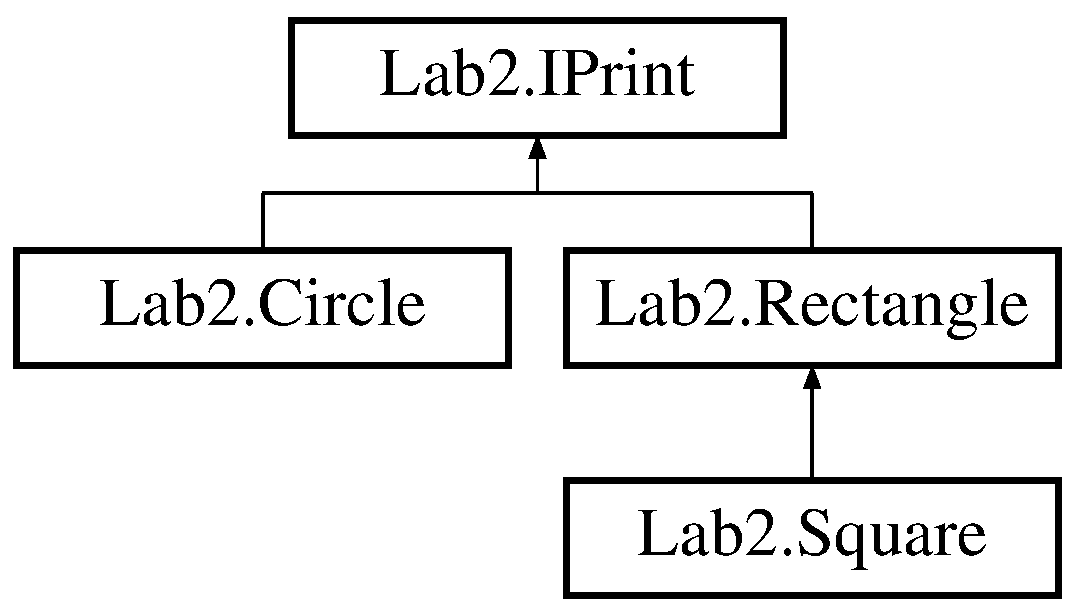
\includegraphics[height=3.000000cm]{interface_lab2_1_1_i_print}
\end{center}
\end{figure}
\subsection*{Открытые члены}
\begin{DoxyCompactItemize}
\item 
void \hyperlink{interface_lab2_1_1_i_print_ab2ab78a92b129513c12b26f473d65c31}{Print} ()
\end{DoxyCompactItemize}


\subsection{Подробное описание}
Интерфейс, для печати на экран 

\subsection{Методы}
\mbox{\Hypertarget{interface_lab2_1_1_i_print_ab2ab78a92b129513c12b26f473d65c31}\label{interface_lab2_1_1_i_print_ab2ab78a92b129513c12b26f473d65c31}} 
\index{Lab2\+::\+I\+Print@{Lab2\+::\+I\+Print}!Print@{Print}}
\index{Print@{Print}!Lab2\+::\+I\+Print@{Lab2\+::\+I\+Print}}
\subsubsection{\texorpdfstring{Print()}{Print()}}
{\footnotesize\ttfamily void Lab2.\+I\+Print.\+Print (\begin{DoxyParamCaption}{ }\end{DoxyParamCaption})}



Замещается в \hyperlink{class_lab2_1_1_circle_a300cdfbc89e35dadfdcd35ff085ffc13}{Lab2.\+Circle} и \hyperlink{class_lab2_1_1_rectangle_a7bc8ce3f09ba299aba57045c396b6b4e}{Lab2.\+Rectangle}.



Объявления и описания членов интерфейса находятся в файле\+:\begin{DoxyCompactItemize}
\item 
\hyperlink{_program_8cs}{Program.\+cs}\end{DoxyCompactItemize}

\hypertarget{class_lab2_1_1_program}{}\section{Класс Lab2.\+Program}
\label{class_lab2_1_1_program}\index{Lab2.\+Program@{Lab2.\+Program}}
\subsection*{Классы}
\begin{DoxyCompactItemize}
\item 
class {\bfseries S\+T\+A\+TE}
\end{DoxyCompactItemize}


Объявления и описания членов класса находятся в файле\+:\begin{DoxyCompactItemize}
\item 
Program.\+cs\end{DoxyCompactItemize}

\hypertarget{class_lab2_1_1_rectangle}{}\section{Класс Lab2.\+Rectangle}
\label{class_lab2_1_1_rectangle}\index{Lab2.\+Rectangle@{Lab2.\+Rectangle}}
Граф наследования\+:Lab2.\+Rectangle\+:\begin{figure}[H]
\begin{center}
\leavevmode
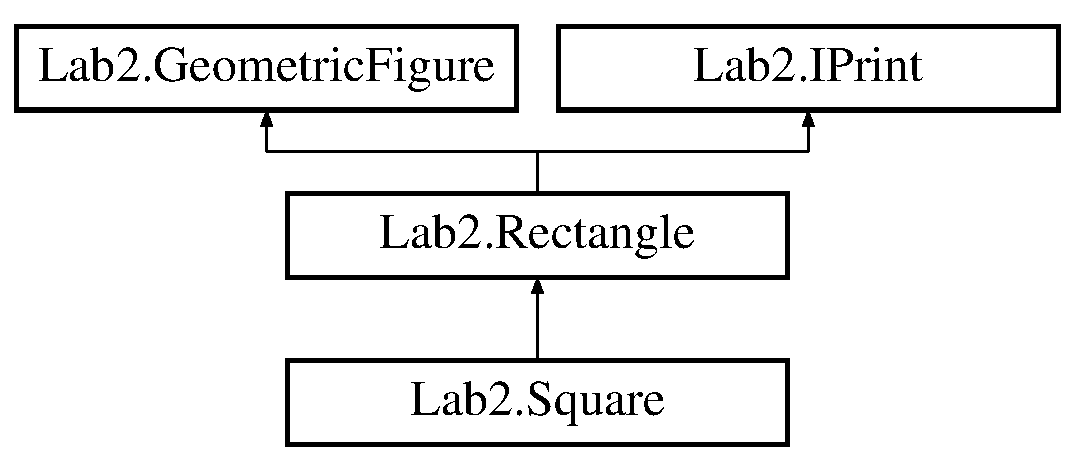
\includegraphics[height=3.000000cm]{class_lab2_1_1_rectangle}
\end{center}
\end{figure}
\subsection*{Открытые члены}
\begin{DoxyCompactItemize}
\item 
\hyperlink{class_lab2_1_1_rectangle_acdb99dd549f51743792cad788e500849}{Rectangle} (double height, double width)
\item 
override double \hyperlink{class_lab2_1_1_rectangle_a3a44a2229aaec3be07a35eb6a167b100}{Area} ()
\item 
override string \hyperlink{class_lab2_1_1_rectangle_a6c03cbd28985951c1c167b51ed47cdd4}{To\+String} ()
\item 
void \hyperlink{class_lab2_1_1_rectangle_a7bc8ce3f09ba299aba57045c396b6b4e}{Print} ()
\end{DoxyCompactItemize}
\subsection*{Открытые атрибуты}
\begin{DoxyCompactItemize}
\item 
double \hyperlink{class_lab2_1_1_rectangle_a94ac15fb6583c21bf4c47bc8cf680aa2}{h} = 0
\begin{DoxyCompactList}\small\item\em Высота \end{DoxyCompactList}\item 
double \hyperlink{class_lab2_1_1_rectangle_a074656a9861271f6b4e17319b7bfc6bb}{w} = 0
\begin{DoxyCompactList}\small\item\em Ширина \end{DoxyCompactList}\end{DoxyCompactItemize}


\subsection{Подробное описание}
Класс прямоугольника 

\subsection{Конструктор(ы)}
\mbox{\Hypertarget{class_lab2_1_1_rectangle_acdb99dd549f51743792cad788e500849}\label{class_lab2_1_1_rectangle_acdb99dd549f51743792cad788e500849}} 
\index{Lab2\+::\+Rectangle@{Lab2\+::\+Rectangle}!Rectangle@{Rectangle}}
\index{Rectangle@{Rectangle}!Lab2\+::\+Rectangle@{Lab2\+::\+Rectangle}}
\subsubsection{\texorpdfstring{Rectangle()}{Rectangle()}}
{\footnotesize\ttfamily Lab2.\+Rectangle.\+Rectangle (\begin{DoxyParamCaption}\item[{double}]{height,  }\item[{double}]{width }\end{DoxyParamCaption})}

Конструктор класса 
\begin{DoxyParams}{Аргументы}
{\em double} & height Задает высоту фигуры \\
\hline
{\em double} & width Задает ширину фигуры \\
\hline
\end{DoxyParams}


\subsection{Методы}
\mbox{\Hypertarget{class_lab2_1_1_rectangle_a3a44a2229aaec3be07a35eb6a167b100}\label{class_lab2_1_1_rectangle_a3a44a2229aaec3be07a35eb6a167b100}} 
\index{Lab2\+::\+Rectangle@{Lab2\+::\+Rectangle}!Area@{Area}}
\index{Area@{Area}!Lab2\+::\+Rectangle@{Lab2\+::\+Rectangle}}
\subsubsection{\texorpdfstring{Area()}{Area()}}
{\footnotesize\ttfamily override double Lab2.\+Rectangle.\+Area (\begin{DoxyParamCaption}{ }\end{DoxyParamCaption})\hspace{0.3cm}{\ttfamily [virtual]}}

Вычисляет площадь фигуры 

Замещает \hyperlink{class_lab2_1_1_geometric_figure_aeb0853b133cedd1d23f5d8a1d73af8a8}{Lab2.\+Geometric\+Figure}.

\mbox{\Hypertarget{class_lab2_1_1_rectangle_a7bc8ce3f09ba299aba57045c396b6b4e}\label{class_lab2_1_1_rectangle_a7bc8ce3f09ba299aba57045c396b6b4e}} 
\index{Lab2\+::\+Rectangle@{Lab2\+::\+Rectangle}!Print@{Print}}
\index{Print@{Print}!Lab2\+::\+Rectangle@{Lab2\+::\+Rectangle}}
\subsubsection{\texorpdfstring{Print()}{Print()}}
{\footnotesize\ttfamily void Lab2.\+Rectangle.\+Print (\begin{DoxyParamCaption}{ }\end{DoxyParamCaption})}

Напечатать основную информацию об объекте в консоль 

Замещает \hyperlink{interface_lab2_1_1_i_print_ab2ab78a92b129513c12b26f473d65c31}{Lab2.\+I\+Print}.

\mbox{\Hypertarget{class_lab2_1_1_rectangle_a6c03cbd28985951c1c167b51ed47cdd4}\label{class_lab2_1_1_rectangle_a6c03cbd28985951c1c167b51ed47cdd4}} 
\index{Lab2\+::\+Rectangle@{Lab2\+::\+Rectangle}!To\+String@{To\+String}}
\index{To\+String@{To\+String}!Lab2\+::\+Rectangle@{Lab2\+::\+Rectangle}}
\subsubsection{\texorpdfstring{To\+String()}{ToString()}}
{\footnotesize\ttfamily override string Lab2.\+Rectangle.\+To\+String (\begin{DoxyParamCaption}{ }\end{DoxyParamCaption})\hspace{0.3cm}{\ttfamily [virtual]}}

Приведение к строке \begin{DoxyReturn}{Возвращает}
string Основная информация об объекте 
\end{DoxyReturn}


Замещает \hyperlink{class_lab2_1_1_geometric_figure_a2f466edc438f43540ead2bc66925ef0a}{Lab2.\+Geometric\+Figure}.



Переопределяется в \hyperlink{class_lab2_1_1_square_ac43e17280bb521a3466a38ec0e4742eb}{Lab2.\+Square}.



\subsection{Данные класса}
\mbox{\Hypertarget{class_lab2_1_1_rectangle_a94ac15fb6583c21bf4c47bc8cf680aa2}\label{class_lab2_1_1_rectangle_a94ac15fb6583c21bf4c47bc8cf680aa2}} 
\index{Lab2\+::\+Rectangle@{Lab2\+::\+Rectangle}!h@{h}}
\index{h@{h}!Lab2\+::\+Rectangle@{Lab2\+::\+Rectangle}}
\subsubsection{\texorpdfstring{h}{h}}
{\footnotesize\ttfamily double Lab2.\+Rectangle.\+h = 0}



Высота 

\mbox{\Hypertarget{class_lab2_1_1_rectangle_a074656a9861271f6b4e17319b7bfc6bb}\label{class_lab2_1_1_rectangle_a074656a9861271f6b4e17319b7bfc6bb}} 
\index{Lab2\+::\+Rectangle@{Lab2\+::\+Rectangle}!w@{w}}
\index{w@{w}!Lab2\+::\+Rectangle@{Lab2\+::\+Rectangle}}
\subsubsection{\texorpdfstring{w}{w}}
{\footnotesize\ttfamily double Lab2.\+Rectangle.\+w = 0}



Ширина 



Объявления и описания членов класса находятся в файле\+:\begin{DoxyCompactItemize}
\item 
\hyperlink{_program_8cs}{Program.\+cs}\end{DoxyCompactItemize}

\hypertarget{class_lab2_1_1_square}{}\section{Класс Lab2.\+Square}
\label{class_lab2_1_1_square}\index{Lab2.\+Square@{Lab2.\+Square}}
Граф наследования\+:Lab2.\+Square\+:\begin{figure}[H]
\begin{center}
\leavevmode
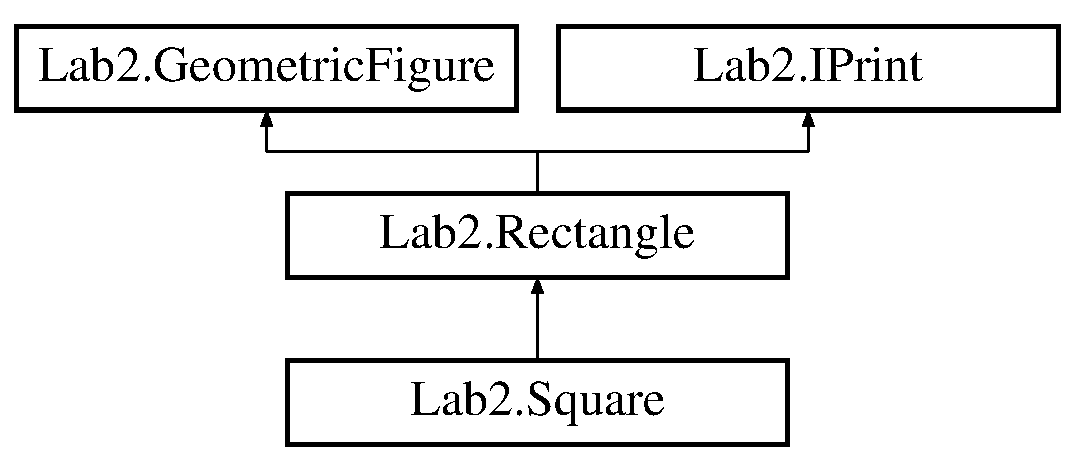
\includegraphics[height=3.000000cm]{class_lab2_1_1_square}
\end{center}
\end{figure}
\subsection*{Открытые члены}
\begin{DoxyCompactItemize}
\item 
\hyperlink{class_lab2_1_1_square_adf14884086bf810bde5cb9dc18e10a82}{Square} (double length)
\item 
override string \hyperlink{class_lab2_1_1_square_ac43e17280bb521a3466a38ec0e4742eb}{To\+String} ()
\end{DoxyCompactItemize}
\subsection*{Дополнительные унаследованные члены}


\subsection{Подробное описание}
Класс квадрата 

\subsection{Конструктор(ы)}
\mbox{\Hypertarget{class_lab2_1_1_square_adf14884086bf810bde5cb9dc18e10a82}\label{class_lab2_1_1_square_adf14884086bf810bde5cb9dc18e10a82}} 
\index{Lab2\+::\+Square@{Lab2\+::\+Square}!Square@{Square}}
\index{Square@{Square}!Lab2\+::\+Square@{Lab2\+::\+Square}}
\subsubsection{\texorpdfstring{Square()}{Square()}}
{\footnotesize\ttfamily Lab2.\+Square.\+Square (\begin{DoxyParamCaption}\item[{double}]{length }\end{DoxyParamCaption})}

Конструктор класса 
\begin{DoxyParams}{Аргументы}
{\em double} & length Задает длину стороны квадрата \\
\hline
\end{DoxyParams}


\subsection{Методы}
\mbox{\Hypertarget{class_lab2_1_1_square_ac43e17280bb521a3466a38ec0e4742eb}\label{class_lab2_1_1_square_ac43e17280bb521a3466a38ec0e4742eb}} 
\index{Lab2\+::\+Square@{Lab2\+::\+Square}!To\+String@{To\+String}}
\index{To\+String@{To\+String}!Lab2\+::\+Square@{Lab2\+::\+Square}}
\subsubsection{\texorpdfstring{To\+String()}{ToString()}}
{\footnotesize\ttfamily override string Lab2.\+Square.\+To\+String (\begin{DoxyParamCaption}{ }\end{DoxyParamCaption})\hspace{0.3cm}{\ttfamily [virtual]}}

Приведение к строке \begin{DoxyReturn}{Возвращает}
string Основная информация об объекте 
\end{DoxyReturn}


Переопределяет метод предка \hyperlink{class_lab2_1_1_rectangle_a6c03cbd28985951c1c167b51ed47cdd4}{Lab2.\+Rectangle}.



Объявления и описания членов класса находятся в файле\+:\begin{DoxyCompactItemize}
\item 
\hyperlink{_program_8cs}{Program.\+cs}\end{DoxyCompactItemize}

\hypertarget{class_lab2_1_1_program_1_1_s_t_a_t_e}{}\section{Класс Lab2.\+Program.\+S\+T\+A\+TE}
\label{class_lab2_1_1_program_1_1_s_t_a_t_e}\index{Lab2.\+Program.\+S\+T\+A\+TE@{Lab2.\+Program.\+S\+T\+A\+TE}}
\subsection*{Открытые атрибуты}
\begin{DoxyCompactItemize}
\item 
const String \hyperlink{class_lab2_1_1_program_1_1_s_t_a_t_e_a7e20c40f4173c5b32eea8e3b8c9a41ea}{Rectangle} = \char`\"{}1\char`\"{}
\item 
const String \hyperlink{class_lab2_1_1_program_1_1_s_t_a_t_e_a38e1a16e8f362a6c14580625b94cc191}{Sqare} = \char`\"{}2\char`\"{}
\item 
const String \hyperlink{class_lab2_1_1_program_1_1_s_t_a_t_e_abfa46dc8209ae33faad2a798dab636ab}{Circle} = \char`\"{}3\char`\"{}
\end{DoxyCompactItemize}


\subsection{Подробное описание}
Класс с константами выбора пользователя 

\subsection{Данные класса}
\mbox{\Hypertarget{class_lab2_1_1_program_1_1_s_t_a_t_e_abfa46dc8209ae33faad2a798dab636ab}\label{class_lab2_1_1_program_1_1_s_t_a_t_e_abfa46dc8209ae33faad2a798dab636ab}} 
\index{Lab2\+::\+Program\+::\+S\+T\+A\+TE@{Lab2\+::\+Program\+::\+S\+T\+A\+TE}!Circle@{Circle}}
\index{Circle@{Circle}!Lab2\+::\+Program\+::\+S\+T\+A\+TE@{Lab2\+::\+Program\+::\+S\+T\+A\+TE}}
\subsubsection{\texorpdfstring{Circle}{Circle}}
{\footnotesize\ttfamily const String Lab2.\+Program.\+S\+T\+A\+T\+E.\+Circle = \char`\"{}3\char`\"{}}

\mbox{\Hypertarget{class_lab2_1_1_program_1_1_s_t_a_t_e_a7e20c40f4173c5b32eea8e3b8c9a41ea}\label{class_lab2_1_1_program_1_1_s_t_a_t_e_a7e20c40f4173c5b32eea8e3b8c9a41ea}} 
\index{Lab2\+::\+Program\+::\+S\+T\+A\+TE@{Lab2\+::\+Program\+::\+S\+T\+A\+TE}!Rectangle@{Rectangle}}
\index{Rectangle@{Rectangle}!Lab2\+::\+Program\+::\+S\+T\+A\+TE@{Lab2\+::\+Program\+::\+S\+T\+A\+TE}}
\subsubsection{\texorpdfstring{Rectangle}{Rectangle}}
{\footnotesize\ttfamily const String Lab2.\+Program.\+S\+T\+A\+T\+E.\+Rectangle = \char`\"{}1\char`\"{}}

\mbox{\Hypertarget{class_lab2_1_1_program_1_1_s_t_a_t_e_a38e1a16e8f362a6c14580625b94cc191}\label{class_lab2_1_1_program_1_1_s_t_a_t_e_a38e1a16e8f362a6c14580625b94cc191}} 
\index{Lab2\+::\+Program\+::\+S\+T\+A\+TE@{Lab2\+::\+Program\+::\+S\+T\+A\+TE}!Sqare@{Sqare}}
\index{Sqare@{Sqare}!Lab2\+::\+Program\+::\+S\+T\+A\+TE@{Lab2\+::\+Program\+::\+S\+T\+A\+TE}}
\subsubsection{\texorpdfstring{Sqare}{Sqare}}
{\footnotesize\ttfamily const String Lab2.\+Program.\+S\+T\+A\+T\+E.\+Sqare = \char`\"{}2\char`\"{}}



Объявления и описания членов класса находятся в файле\+:\begin{DoxyCompactItemize}
\item 
\hyperlink{_program_8cs}{Program.\+cs}\end{DoxyCompactItemize}

\chapter{Файлы}
\hypertarget{_program_8cs}{}\section{Файл Program.\+cs}
\label{_program_8cs}\index{Program.\+cs@{Program.\+cs}}
\subsection*{Классы}
\begin{DoxyCompactItemize}
\item 
class \hyperlink{class_lab1_1_1_program}{Lab1.\+Program}
\end{DoxyCompactItemize}
\subsection*{Пространства имен}
\begin{DoxyCompactItemize}
\item 
namespace \hyperlink{namespace_lab1}{Lab1}
\end{DoxyCompactItemize}

%--- End generated contents ---

% Index
\backmatter
\newpage
\phantomsection
\clearemptydoublepage
\addcontentsline{toc}{chapter}{Алфавитный указатель}
\printindex

\end{document}
